\documentclass{article}
\usepackage[utf8]{inputenc}
\usepackage{tikz}
\usepackage{pgfplots, pgfplotstable}
\usepackage{caption}

\title{MC886 - Machine learning \\ Exercise 2}
\author{Rafael Almeida Erthal Hermano\\RA 121286}
\date{March 2014}

\begin{document}

\maketitle
\newpage

\section{Results}
\subsection{Results of numbers 1 and 7}
The algorithm was tested with 80 images and the matches for each number of dimensions and neighbors are:

\begin{table}[h]
\begin{tabular}{|l|l|l|l|}
\hline
Neighbors & 4096 dimensions & 100 dimensions & 40 dimension \\ \hline
1         & 65 & 65 & 63 \\ \hline
3         & 57 & 58 & 65 \\ \hline
5         & 53 & 60 & 64 \\ \hline
11        & 49 & 55 & 60 \\ \hline
17        & 47 & 56 & 61 \\ \hline
21        & 46 & 56 & 59 \\ \hline
\end{tabular}
\end{table}

Comparing the results with the following graph.

\begin{center}
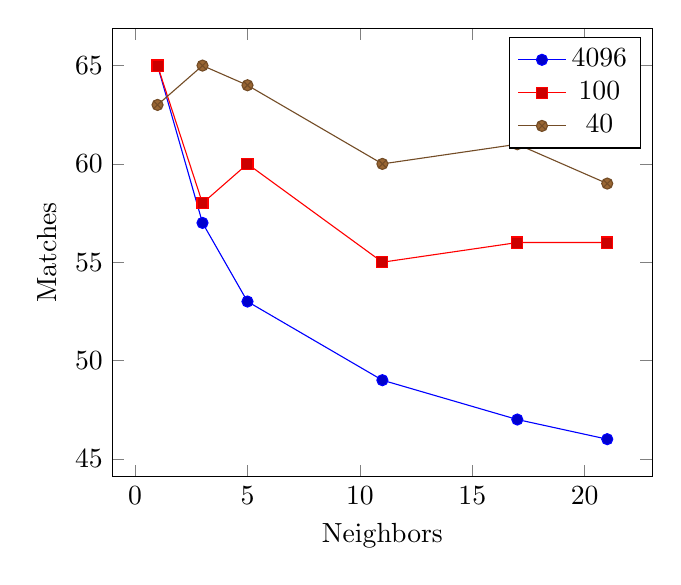
\begin{tikzpicture}
    \begin{axis}[xlabel=Neighbors, ylabel=Matches]
    \addplot coordinates {
        (1, 65 )
        (3, 57 )
        (5, 53 )
        (11, 49 )
        (17, 47 )
        (21, 46 )
    };
    \addlegendentry{4096}
    \addplot coordinates {
        (1, 65 )
        (3, 58 )
        (5, 60 )
        (11, 55 )
        (17, 56 )
        (21, 56 )
    };
    \addlegendentry{100}
    \addplot coordinates {
        (1, 63 )
        (3, 65 )
        (5, 64 )
        (11, 60 )
        (17, 61 )
        (21, 59 )
    };
    \addlegendentry{40}
    \end{axis}
\end{tikzpicture}
\end{center}

The best solutions where with 1 neighbor and 4096 or 100 dimensions. But with 40 dimensions, the average for all combinations of neighbors is higher so using 40 dimensions is better because we can use more neighbors and avoid overfiting.
\newpage

\subsection{Results of numbers 4 and 9}
The algorithm was tested with 50 images and the matches for each number of dimensions and neighbors are:

\begin{table}[h]
\begin{tabular}{|l|l|l|l|}
\hline
Neighbors & 4096 dimensions & 100 dimensions & 40 dimension \\ \hline
1         & 42 & 39 & 44 \\ \hline
3         & 39 & 36 & 42 \\ \hline
5         & 33 & 33 & 41 \\ \hline
11        & 34 & 38 & 37 \\ \hline
17        & 31 & 36 & 38 \\ \hline
21        & 33 & 32 & 34 \\ \hline
\end{tabular}
\end{table}

Comparing the results with the following graph.

\begin{center}
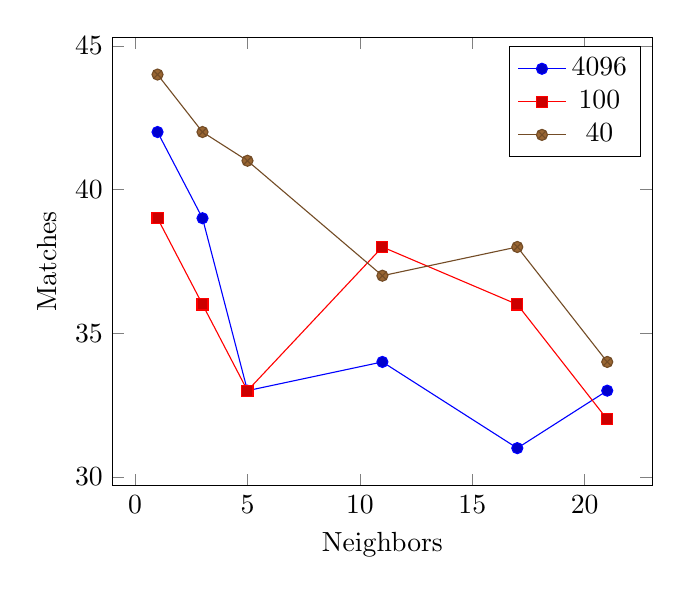
\begin{tikzpicture}
    \begin{axis}[xlabel=Neighbors, ylabel=Matches]
    \addplot coordinates {
        (1, 42 )
        (3, 39 )
        (5, 33 )
        (11, 34 )
        (17, 31 )
        (21, 33 )
    };
    \addlegendentry{4096}
    \addplot coordinates {
        (1, 39 )
        (3, 36 )
        (5, 33 )
        (11, 38 )
        (17, 36 )
        (21, 32 )
    };
    \addlegendentry{100}
    \addplot coordinates {
        (1, 44 )
        (3, 42 )
        (5, 41 )
        (11, 37 )
        (17, 38 )
        (21, 34 )
    };
    \addlegendentry{40}
    \end{axis}
\end{tikzpicture}
\end{center}

The best solution was with 1 neighbor and 40 dimensions, and the average of matches is higher with 40 dimensions so its better to apply PCA and use 40 dimensions and maybe a higher number of neighbors to avoid overfiting.

\end{document}